  Dieses Kapitel behandelt die Evaluation der Java Web Frameworks. Es wird die
  kombinierte Methode aus dem Kapitel 
  \ref{chapter:MethodenZurEntscheidungsfindungBeiEinerEvaluation}
  (\nameref{chapter:MethodenZurEntscheidungsfindungBeiEinerEvaluation}, S.
  \pageref{chapter:MethodenZurEntscheidungsfindungBeiEinerEvaluation}ff)
  angewendet. Mit der definition von sinnvollen Rahmenbedingungen soll die
  Evaluation durchgeführt und das Resultate in Form einer Rangliste vorgelegt
  werden.
    
  \section{Rahmenbedingungen für die Evaluierung}
  
  Über Soll-Kriterien und KO-Kriterien werden die Rahmenbedingungen für die
  Evaluierung festgelegt. Die Soll-Kriterien wiederspiegeln die Anforderungen,
  welche an ein Java Web Framework gestellt werden. Die KO-Kriterien dienen zum
  Ausschluss, nicht geeigneter Frameworks.

  \subsection{Soll-Kriterien}
  
  Die Eignung, der zu evaluierenden Java Web Frameworks, wird durch eine Menge
  von Soll-Kriterien bestimmt. Die Soll-Kriterien bestimmen die Anforderungen,
  welche erfüllt werden sollen. Die Anforderungen stammen von einer
  Projektgruppe der Hochschule für Technik und Wirtschaft Berlin. Die
  Soll-Kriterien werden für den Einsatz in der \ac{ZKB} priorisiert.
  
  Soll-Kriterien sind Vorgaben, die möglichst weitgehend Erfüllt werden sollen.
  Wenn ein solches Kriterium nicht erfüllt werden kann, schliesst das die
  Alternative nicht aus. Jedem Soll-Kriterium wird für die Identifikation eine
  eindeutige ID vergeben. Die ID setzt sich folgendermassen zusammen: 
  \{Soll\}-\{Laufnummer\}.
  
  \subsubsection{Anforderungen an Web Frameworks nach AgileLearn}
  
  Eine Projektgruppe namens AgileLearn von der Hochschule für Technik und
  Wirtschaft Berlin befasst sich mit dem Thema Web Frameworks. Die
  Projektgruppe hat sich die Frage gestellt: ``\begin{itshape}Welche
  Anforderungen müssen bei der Wahl eines Webframeworks berücksichtigt
  werden?\end{itshape}''\footnote{Zitat von Raoul Jaeckel, siehe
  \cite{AnforderungenAnWebframeworks}}. Aus der Fragestellung heraus, haben sie
  18 Anforderungen an ein Web Framework ausgearbeitet, welche öffentlich in
  einem Google-Doc\footnote{Ein Service von Google um Dokumente öffentlich zu
  bearbeiten.} ersichtlich sind.
  
  Folgende Anforderungen stammen aus dem Dokument ``\begin{itshape}18
  Anforderungen an Webframeworks -
  OpenDoc\end{itshape}'', siehe \cite{AnforderungenAnWebframeworks}, und werden
  im Anhang \ref{chapter:18AnforderungenNachAgileLearn}
  (\nameref{chapter:18AnforderungenNachAgileLearn}, S.
  \pageref{chapter:18AnforderungenNachAgileLearn}ff) zusammengefasst und mit
  einer ID versehen.

  \subsection{KO-Kriterien}
  
  Anhand einer Menge von KO-Kriterien wird die Auswahl der Alternativen
  eingeschränkt. Die KO-Kriterien sind aus dem \begin{itshape}Handbuch der
  IT-Architektur\end{itshape}, siehe \cite{ZkbHandbuchDerItArchitektur}, der
  \ac{ZKB} entnommen. Die Namensgebung in dem Handbuch unterscheidet sich
  leicht, es wird nicht von KO-Kriterien, sondern von Grundsätzen gesprochen.
  
  KO-Kriterien sind Vorgaben, welche zwingend erfüllt sein müssen. Falls ein
  Kriterium nicht erfüllt werden kann, fällt die Entscheidung auf diese
  Alternative negativ aus. Jedem KO-Kriterium wird für die Identifikation eine
  eindeutige ID vergeben. Die ID setzt sich folgendermassen zusammen: 
  \{KO\}-\{Laufnummer\}.

  \subsubsection{Grundsätze aus der IT-Architektur der Zürcher Kantonalbank}
  
  Ein Grundsatz wird im Handbuch wer IT-Architektur wie folgt definiert:
  \newline
  
  ``\begin{itshape}Es sind Grundsätze definiert, nach denen sich die Baupläne
  der IT-Systeme zu richten haben. Die Grundsätze sind ein Regelwerk mit
  Weisungscharakter.\end{itshape}''
  \footnote{\cite{ZkbHandbuchDerItArchitektur} Kapitel 1.3 - \begin{itshape}Was
  ist die IT-Architektur der ZKB\end{itshape}, Seite 11}
  \newline

  \noindent
  Dabei gibt es eine Hintertür:
  \newline

  ``\begin{itshape}Grundsätze sind verbindliche Vorgaben (Konventionen), von
  denen nur in begründeten Ausnahmen abgewichen werden kann.\end{itshape}''
  \footnote{\cite{ZkbHandbuchDerItArchitektur} Kapitel 1.8 -
  \begin{itshape}Leseanleitung\end{itshape}, Seite 14}
  \newline
  
  \noindent
  Das Dokument wurde analysiert und alle Grundsätze, welche für diese
  Diplomarbeit relevanten sind, werden im Anhang
  \ref{chapter:GrundsaetzeDerZkbItArchitektur}
  (\nameref{chapter:GrundsaetzeDerZkbItArchitektur}, S.
  \pageref{chapter:GrundsaetzeDerZkbItArchitektur}ff) aufgelistet und mit einer
  ID versehen.

  \section{Priorisierung der Soll-Kriterien}
  
  Da 18 Soll-Kriterien definiert wurden und diese in jeder Alternative 
  untersucht werden müssten, würde das den Rahmen der Diplomarbeit sprengen.
  Desshalb sollen die Soll-Kriterien in eine Hirarchie entsprechend ihrer
  Wichtigkeit für die \ac{ZKB} aufgeteilt werden. Es sollen nur die
  ``wichtigen'' Soll-Kriterien in die Evaluation mit einbezogen werden. Die
  Hirarchie wird desshalb in drei Gruppen aufgeteilt:
  
  \begin{itemize}
    \item Wichtig
    \item Nice to have
    \item Unwichtig
  \end{itemize}
  
  \noindent

  
  \subsection{Wichtige Aspekte im Software-Lebenszyklus für die ZKB}
  
  \begin{description}
    \item[Sicherheit]
    Nur eine Bank, die als sicher gilt, hat das Vertrauen der Kunden und somit
    Erfolg in ihrem Geschäft.
    \item[Kosten]
    Die laufenden Kosten sollen so tief wie möglich gehalten werden. Gemäss
    Abbildung \ref{img:softwareLifecycleCost} liegen die Hauptkosten im
    Software-Lebenszyklus bei der Maintenance-Phase. Somit können die Kosten für
    requirements Engineering, Design, Programming und Integration vernachlässigt
    werden.
    \item[Ressourcen]
    Damit Software entwickelt und gewartet werden kann, wird die Verfügbarkeit
    von qualifizierten Ressourcen benötigt.
    \item[Image]
    Um sich von der Konkurenz abzuheben wird ein Image aufgebaut das sich
    zeitgemäss, flexibel und inovativ präsentieren soll, siehe
    \cite{WillkommenBeiDerZkb} S. 34ff.
  \end{description}
  
  \begin{figure}[ht]
    \begin{center}
      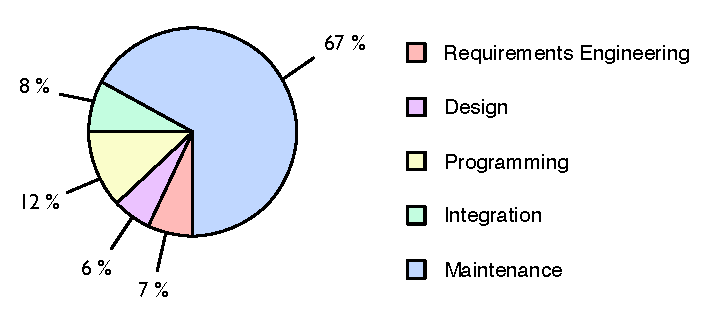
\includegraphics[width=0.7\textwidth]{./image/softwareLifeCycleCost.pdf}
      \caption{Ungefähre relative Kosten der Phasen des Software-Lebenszyklus
      (nach \cite{SoftwareEngineering} S. 11 und
      \cite{SoftwareLifeCycleModels})}
      \label{img:softwareLifecycleCost}
    \end{center}
  \end{figure}
  
  \begin{table}[h!]
    \sffamily 
    \begin{center}
      \begin{threeparttable}
        \begin{tabular}{p{9cm}cccc}
          \toprule
          Anforderung & (Si) & (Ko) & (Re) & (Im)\\
          \midrule
          \ref{itm:Soll-01} & ++ &    &    &    \\
          \ref{itm:Soll-02} & +  &    &    &    \\
          \ref{itm:Soll-03} &    & ++ &    &    \\
          \ref{itm:Soll-04} &    & +  &    &    \\
          \ref{itm:Soll-05} &    &    &    &    \\
          \ref{itm:Soll-06} & +  & ++ &    & ++ \\
          \ref{itm:Soll-07} &    &    &    &    \\
          \ref{itm:Soll-08} &    &    &    &    \\
          \ref{itm:Soll-09} &    &    &    &    \\
          \ref{itm:Soll-10} &    &    &    &    \\
          \ref{itm:Soll-11} &    &    &    &    \\
          \ref{itm:Soll-12} &    & ++ &    &    \\
          \ref{itm:Soll-13} &    &    & ++ &    \\
          \ref{itm:Soll-14} &    & +  &    &    \\
          \ref{itm:Soll-15} &    &    &    &    \\
          \ref{itm:Soll-16} &    &    &    &    \\
          \ref{itm:Soll-17} &    &    & +  &    \\
          \ref{itm:Soll-18} &    &    &    & ++ \\
          \bottomrule
        \end{tabular}
        \caption{Wie wichtig sind die Soll-Kriterien für die ZKB.}
        \label{tab:kosolidierungDerSollKriterien}
        \medskip 
        %\footnotesize\textbf{Legende:}\smallskip 
        \begin{tablenotes}[++]\footnotesize 
          \item[(Si)] Sicherheit 
          \item[(Ko)] Kosten in der Maintenance Phase des Software-Lebenszyklus
          \item[(Re)] Ressourcen 
          \item[(Im)] Image
          \item[++] hat grossen Einfluss
          \item[+] hat Einfluss
        \end{tablenotes}
      \end{threeparttable}
    \end{center}
  \end{table}
  
  \noindent
  Es soll eine Konsolidierung statt finden, zwischen den 18 Soll-Kriterien und
  den wichtigen Aspekten im Software-Lebenszyklus für die \ac{ZKB}. Die
  Konsolidierung wird in der Tabelle \ref{tab:kosolidierungDerSollKriterien}
  gezeigt. Die Soll-Kriterien mit zwei oder mehr + werden als ``wichtig'', mit
  einem + als ``nice to have'' und ohne + als ``nicht wichtig'' priorisiert. Die
  Gründe für die Priorisierung soll anschliessend erläutert werden.
  
  \subsection{Wichtig}
  
  \begin{description}
  \item[Soll-01 - Zugriffskontrolle 
  (Authentifizierung/Authorisation/Rollenverwaltung)]
  Auf die Sicherheit von Applikationen in einer Bank wird grossen Wert
  gelegt. Mit einer genügenden Authentifizierung, Authorisation und
  Rollenverwalung, kann eine Applikation sicher implementiert werden.
  
  \item[Soll-03 - Modulare Architektur]
  Um wärend der Maintenance-Phase des Software Lebenszyklus notwendige
  Anpassungen an einer Applikation machen zu können, ist eine modulare
  Architekur von grossem Vorteil. Zudem ist das auch wärend der
  Entwicklungs-Phase hilfreich.
  
  \item[Soll-06 - Testing]
  Um wärend der Maintenance-Phase des Software-Lebenszyklus notwendige
  Anpassungen an einer Applikation machen zu können, ist ein gutes Testing von
  grossem Vorteil. Das Testing hat auch einen grossen Einfluss auf das Image,
  denn wer möchte schon fehlerhafte Software verwenden. Durch eine gute
  Testbasis, kann auch die Sicherheit einer Applikation gesteigert werden.
  
  \item[Soll-12 - Dokumentation]
  Eine saubere und verständliche Dokumentation eines Web Application Frameworks
  ist das A und O um während allen Software-Lebenszyklen effizient arbeiten zu
  können. Ein Web Application Framework mit einer brillianten Dokumentation hat
  bestimmt höhere Chancen sich längerfristig am Markt durchzusetzten.
  
  \item[Soll-13 - Community]
  Damit die notwendigen Ressourcen, für die Umsetztung und Wartung eines
  Software-Projekts gefunden werden, wird eine entsprechend grosse Community
  benötigt. Wenn die Community genügend gross ist, kann man davon ausgehen,
  dass auch in der Zukunft noch genügend Ressourcen in diesem Bereich
  erreichbar sind.
  
  \item[Soll-18 - AJAX-Unterstützung]
  In der Zeit von Google Mail, Facebook und Twitter wird die Verwendung von
  \ac{Ajax} unterstützten Web Applikationen zur Gewohnheit. Um mit einer Web
  Applikation ein zeitgemässes, flexibles und innovatives Image vermitteln zu
  können, sollten diese mit Ajax-Unterstütztung gebaut werden.
  
  \end{description}
  
  \subsection{Nice to have}
  
  \begin{description}
  \item[Soll-02 - Form-Validierung]
  Eine saubere Form-Validierung gehört zu den notwendigen Werkzeugen, um eine
  sichere Web Applikation zu entwickeln. Dennoch kann durch gutes Testing und
  eine sichere Zugriffskontrolle der selbe Effekt erzielt werden.
  
  \item[Soll-04 - Schnittstellen und Webservices]
  Durch die breite Unterstützung von Schnittstellen und Webservice Technologien
  in der Java Welt, muss ein Web Framework dies nicht schon von Haus aus
  mitbringen. Fall es doch vorhanden ist, um so besser.
  
  \item[Soll-14 - IDE-Unterstuetzung]
  Eine IDE-Unterstützung ist zu präferieren, soll aber kein Hinderniss für den
  Einsatz eines guten Web Frameworks sein.
  
  \item[Soll-17 - Lernkurve fuer EntwicklerInnen]
  Durch die Unterstützung einer soliden Community und einer guten Dokumentation
  kann die Lernkurve beträchtlich beeinflusst werden.
  
  \end{description}
  
  \subsection{Unwichtig}
  
  \begin{description}
  \item[Soll-05 - MVC-Entwurfsmuster]
  Das \ac{MVC} Konzept ist sicher gut, sollte aber nicht eine Anforderung an ein
  Web Framework sein, da es ebenbürdige Alternativen gibt, eine nennenswerte währe
  \ac{MVP}.
  
  \item[Soll-07 - Internationalisierung und Lokalisierung]
  Die \ac{ZKB} hat ihr Geschäftsfeld im Kanton Zürich. Somit ist eine
  Internationalisierung und Lokalisierung nicht wirklich nötig. Da die \ac{ZKB}
  im Auftrag des Kantons handelt, gehe ich davon aus, dass sich das nicht so
  schnell ändern wird.
  
  \item[Soll-08 - Object Relational Mapping (ORM)]
  In der Java Welt git es viele \ac{ORM} Lösungen, welche sich in den Jahren
  durchgesetzt haben, ein paar nennenswerte sind Hibernate, TopLink und
  EclipseLink. Da es Sache des Applikationsservers ist, welches \ac{ORM}
  verwendet wird, stellt dies keine Anforderung an ein Java Web Framework.
  
  \item[Soll-09 - Scaffolding / Rapid Prototyping]
  Scaffolding und Rapid Prototyping kann in der Programmier-Phase des
  Software-Lebenszyklus die Arbeit erleichtern. In der Maintenance-Phase
  ergibt sich daraus kein Benefit.
  
  \item[Soll-10 - Caching]
  Caching kann bei Webseiten mit viel statischen Content die Datenmenge, die
  übertragen wird, enorm reduzieren. Bei Business-Applikationen, die über eine
  Rollenverwaltung verfügen, sind die Daten die übertragen werden, meistens sehr
  individuell. Somit besteht keine grosse Nachfrage nach Caching
  
  \item[Soll-11 - View-Engine]
  Da Java eine Objekt Orientierte Sprache ist, wird das schon von der Sprache
  her unterstützt.
  
  \item[Soll-15 - Kosten fuer Entwicklungswerkzeuge]
  Die Kosten der Entwicklungswerkzeuge haben keinen Einfluss auf die
  Maintenance-Phase des Software-Lebenszyklus. Zudem gibt es genügend \acp{IDE}
  für Java, die Open Source sind. Ein Paar nennenswerte sind Eclipse, NetBeans
  und IntelliJ.
  
  \item[Soll-16 - Eignung fuer agile Entwicklung]
  Die Ansätze von Scrum und extreme Programming werden in der \ac{ZKB} je länger
  je mehr angewendet. Dennoch hat das keinen Einfluss auf die Maintenance-Phase
  des Software-Lebenszyklus.
  
  \end{description}
  
  \section{KO-Kriterien die nicht beachtet werden sollen}
  
  Damit die Durchführung der Evaluation einen Sinn ergibt, sollen einige
  KO-Kriterien nicht beachtet werden. In Absprache mit dem Fachbetreuer der
  \ac{ZKB} betrifft das folgende KO-Kriterien, die im Rahmen der Diplomarbeit
  nicht berücksichtigt werden:
  
  \begin{itemize}
    \item \ref{itm:KO-09} - Für Java-Applikationen (Internet, Extranet und
    Intranet) wird das ZIP-Framework eingesetzt.
    \item \ref{itm:KO-16} - Die Internet-Applikationen funktionieren auch
    eingeschränkt, ohne dass die Skript-Funktion im Browser aktiviert ist.
    \item \ref{itm:KO-20} - Für Ultra Thin Clients bzw. Browser-basierende
    Applikationen muss das aktuelle, Struts-basierende HTML-Client-Framework
    der ZKB Internet Plattform verwendet werden.
  \end{itemize}
  
  \section{Auswahl der Java Web Frameworks}
  
  Es sollen vier Java Web Frameworks für die Evaluation ausgewählt werden. Ein
  Java Web Framework, das in Frage kommt, wird Alternative genannt. Jede
  Alternative wird mit einer ID in der Form \{A\}-\{Laufnummer\} versehen.
  
  \subsection{Begründung}
  
  Es soll für jede Alternative der Grund der Wahl erläutert werden. In Absprache
  mit dem Projektbetreuer sollen aus den verschiednen Typen von Java Web
  Frameworks jeweils eines gewählt werden. Es wurden folgende Typen definiert:
  
  \begin{itemize}
    \item \ac{RIA} - Frameworks
    \item MVC - Frameworks
    \item Java Script/HTML/CSS - Cross-Compiler Frameworks
    \item In der \ac{ZKB} bereits eingesetzte Frameworks
  \end{itemize}
  
  \subsubsection{A-1 - ULC, Canoo RIA Suite}
  
  ULC, Canoo RIA Suite zählt zu den \ac{RIA} Frameworks. Gemäss Kick-off
  Protokoll Beschluss soll dieses Framework als Alternative gewählt werden.
  Zudem wird die ULC, Canoo RIA Suite in den schweizer Banken Credit Suisse und
  UBS eingesetzt.
  
  \subsubsection{A-2 - Struts 1.3.10 mit ZIP-Framework}
  
  MVC - Framework, das in der ZKB bereits eingesetzt wird.
  
  \subsubsection{A-3 - Vaadin 6.5.7}
  
  Vaadin zählt zu den Java Script/\ac{HTML}/\ac{CSS} - Cross-Compiler Frameworks
  und baut auf \ac{GWT} auf.
  
  \subsubsection{A-4 - Apache Wicket 1.4.17}
  
  Ein Framework das in der ZKB bereits eingesetzt wird. An dieser Stelle ist zu
  erwähnen, dass der Einsatz aufgrund von Ausnahmegenehmigungen eingesetzt
  werden darf. Diese müssten im Falle einer erfolgreichen Evaluation ebenfalls
  beantragt werden.
  
  \section{Prüfen der zu beachtenden KO-Kriterien}
  
  Es soll eine Prüfung aller Java Web Frameworks statt finden, ob ein solches
  gegen definierte KO-Kriterien verstösst. Falls das der Fall ist, wird das
  Framework von der Evaluation ausgeschlossen. Falls das nicht zutrifft, wird
  das Framework in die Evaluation miteinbezogen, siehe Abbildung
  \ref{img:ablaufEvaluation}.
  
  In Absprache mit dem Fachbetreuer der \ac{ZKB} gibt es gewisse KO-Kriterien,
  die im Rahmen der Diplomarbeit ausser Kraft treten, diese sollen nicht
  beachtet werden. Das Resultat wird in der Tabelle
  \ref{tab:gefundeneKOKriterien} dargestellt.
  \newline
  
  \begin{table}[!h]
    \sffamily 
    \begin{center}
      \begin{tabular}{lcc}
        \toprule
        Java Web Framework & Verstoss gg KO-Kriterium & Ausschluss\\
        \midrule
        A1 - ULC, Canoo RIA Suite & \ref{itm:KO-18} & Ja\\
        & \ref{itm:KO-19} &\\
        A2 - Struts 1.3.10 mit ZIP-Framework & - & Nein\\
        A3 - Vaadin 6.5.7 & - & Nein\\
        A4 - Apache Wicket 1.4.17 & - & Nein\\
        \bottomrule
      \end{tabular}
      \caption{Verstösse gegen KO-Kriterien}
      \label{tab:gefundeneKOKriterien}
    \end{center}
  \end{table}

  \subsection{A-1 - ULC, Canoo RIA Suite - KO-Kriterien gefunden}
  
  Leider wurde wärend der Analyse festgestellt, dass die ULC, Canoo RIA Suite
  nur in einer Java Virtual Machine\footnote{Die Java Virtual Machine ist der
  Teil der \ac{JRE}, der für die Ausführung des Java-Bytecodes verantwortlich
  ist, siehe \cite{JavaVirtualMachine}.} lauffähig ist. Das wird über die
  Technik von Java-Web-Start\footnote{Java-Web-Start ist eine Technik von
  Oracle (damals entwickelt von Sun Microsystems), die es ermöglicht, Java-Anwendungen
  über das Internet mit nur einem Klick zu starten. Im Unterschied zu
  Java-Applets benötigen Java-Web-Start-Anwendungen keinen Browser, um ablaufen
  zu können, siehe \cite{JavaWebStart}.} oder mit der Hilfe von einem
  Java-Applet\footnote{Ein Java-Applet ist ein Computerprogramm, das in der
  Programmiersprache Java verfasst wurde und normalerweise in einem Webbrowser
  ausgeführt wird, siehe \cite{JavaApplet}.} vollbracht. Das ist ersichtlich im
  ULC Architektur Guide, siehe \cite{ULCArchitectureGuide} S. 18. Damit
  verstösst diese Alternative gegen die KO-Kriterien \ref{itm:KO-18} und
  \ref{itm:KO-19}. Aufgrund des Vorgehens aus der Abbildung
  \ref{img:ablaufEvaluation} wird diese Alternative aus der Evaluation
  ausgeschlossen.
  
  Der Client könnte auch als standalone Client implementiert oder in einen
  bestehenden Client integriert werden. Das nützt nichts, da diese Situation
  bereits mit den Java Swing Clients besteht, und abgelöst werden soll.
  
  Falls sich die Grundsätze der IT-Architektur der \ac{ZKB} in der Zunkunft
  dahingehend ändern, dass Java Web Start oder Java Applets verwendet werden
  dürften, stellt die ULC, Canoo RIA Suite ein gute Alternative zur Ablösung
  bestehender Swing Applikationen. Die Eignung müsste zu diesem Zeitpunkt neu
  geprüft werden.
    
  \section{Gewichtete Nutzwertanalyse mit dem Analytic Hirarchy Process}
  
  Es sollen die Soll-Kriterien, auf welche die Frameworks verglichen werden,
  bestimmt werden. Danach soll nach der Methode des \ac{AHP} die Gewichtung der
  Soll-Kriterien vorgenommen und, zur Berechnung der Nutzwertanalyse,
  verwendet werden. Für jede mögliche Alternative soll der Erfüllungsgrad der
  Soll-Kriterien bestimmt und, zur Berechnung der Nutzwertanalyse, vewendet
  werden. Das Resultat der Nutzwertanalyse soll dargestellt werden.
  
  \subsection{Bestimmen der Kriterien}
  
  Die Kriterien, welche in die Evaluation miteinbezogen werden, und somit für
  jede Alternative untersucht werden soll, sind die ``wichtigen''
  Soll-Kriterien:
  
  \begin{itemize}
    \item Soll-01 - Zugriffskontrolle 
    (Authentifizierung/Authorisation/Rollenverwaltung)
    \item Soll-03 - Modulare Architektur
    \item Soll-06 - Testing
    \item Soll-12 - Dokumentation
    \item Soll-13 - Community
    \item Soll-18 - AJAX-Unterstützung
  \end{itemize}
  
  \subsection{Bestimmen der Gewichte mit dem Analytic Hirarchy Process}
  
  Die Bestimmung der Gewichte wird über die Methode des \ac{AHP} gemacht. Für
  den Vergleich der Soll-Kriterien wird die Frage gestellt:
  \begin{itshape}``Wie wichtig ist das Soll-Kriterium für die
  \ac{ZKB}?''\end{itshape}.
  
  Es werden nur alle ``wichtigen'' Soll-Kriterien miteinander verglichen. Die
  Vergleichsmatrix und die daraus resultierende Gewichtung ist in der Tabelle
  \ref{tab:gewichtungDerSollKriterien} und der Abbildung
  \ref{img:gewichtungSollKriterien} ersichtlich. Für die Werte in der
  Vergleichsmatix wird die Skala der Vergleichsgrad, siehe Tabelle
  \ref{tab:vergleichsgrade}, verwendet. Die gewählten Werte wurden vom
  Studenten, im Sinne der \ac{ZKB}, vergeben. Um eine objektivere Vergabe der
  Punkte zu erhalten, müssten die erläuterten Ansätze\footnote{Es gibt sicher
  noch weitere Ansätze die nicht aufgeführt wurden, welche die Qualität der
  Gewichtung verbessern würden.} aus dem Abschnitt
  \ref{subsection:VerbesserungDerGewichtung}
  \nameref{subsection:VerbesserungDerGewichtung} (auf Seite
  \pageref{subsection:VerbesserungDerGewichtung}) angewendet werden, auf deren
  Einsatz im Rahmen der Diplomarbeit verzichtet wurde.
  
  Um die Gewichte anhand der erstellten Vergleichsmatix zu berechnen, wurde das
  Java Programm JAHP 2.1 verwendet.
  
  Der Inkonsistenzfaktor beträgt 0.04754 und ist somit sehr klein. Die
  getroffenen Annahmen der Gewichtung sollten desshalb aussagekräftig sein.
  \newline
  
  \begin{table}[!h]
    \sffamily 
    \begin{center}
      \begin{tabular}{r|cccccc|r}
        \toprule
        Vergleich & Soll-01 & Soll-03 & Soll-06 & Soll-12 & Soll-13 & Soll-18
        & Gewichtung\\
        \midrule
        Soll-01 & 1 & 5 & 3 & 5 & 5 & 3 & 34.81 \%\\
        Soll-03 & $\frac{1}{5}$ & 1 & $\frac{1}{3}$ & 1 & 1 & $\frac{1}{5}$ &
        5.91 \%\\
        Soll-06 & $\frac{1}{3}$ & 3 & 1 & 3 & 3 & 1 & 17.93 \%\\
        Soll-12 & $\frac{1}{5}$ & 1 & $\frac{1}{3}$ & 1 & $\frac{1}{3}$ &
        $\frac{1}{5}$ & 4.85 \% \\
        Soll-13 & $\frac{1}{5}$ & 1 & $\frac{1}{3}$ & 3 & 1 & $\frac{1}{5}$ &
        9.07 \%\\ Soll-18 & $\frac{1}{3}$ & 5 & 1 & 5 & 5 & 1 & 27.43 \%\\
        \bottomrule
      \end{tabular}
      \caption{Vergleichsmatrix der Soll-Kriterien nach der Methode des AHP.}
      \label{tab:gewichtungDerSollKriterien}
    \end{center}
  \end{table}
  
  \begin{figure}[ht]
    \begin{center}
      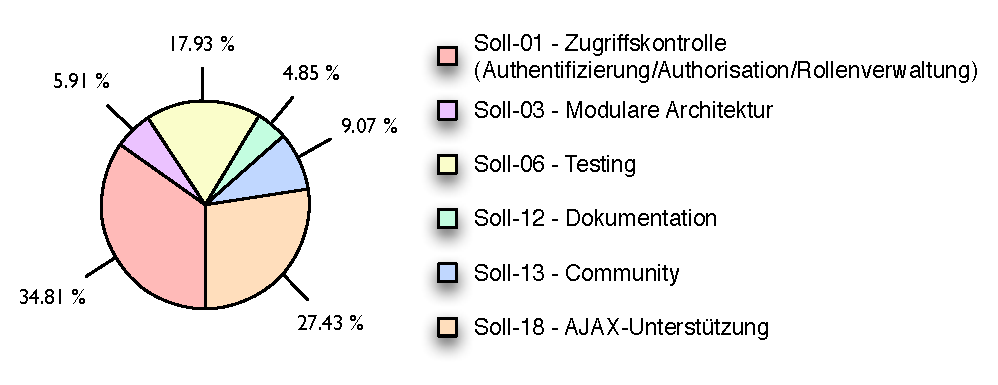
\includegraphics[width=0.95\textwidth]{./image/gewichtungSollKriterien.pdf}
      \caption{Gewichtung der Soll-Kriterien nach der Methode des AHP}
      \label{img:gewichtungSollKriterien}
    \end{center}
  \end{figure}
  
  \subsection{Bestimmen des Erfüllungsgrades}
  
  Für die Werte zur Bestimmung der Erfüllungsgrade wird die Skala der
  Erfüllungsgrade, siehe Tabelle \ref{tab:erfuellungsgrade}, verwendet. Die
  Begründung der gegebenen Punkt wird für jeden Punkt erläutert.
  
  \subsection{A-1 - ULC, Canoo RIA Suite}
  
  ULC, Canoo Ria Suite wurde aufgrund der KO-Kriterien \ref{itm:KO-18} und
  \ref{itm:KO-19} aus der Evaluation ausgeschlossen.
  
  \subsection{A-2 - Struts 1.3.10 mit ZIP-Framework}
  
  Das Ergebnis der Nutzwertanalyse ist in der Tabelle \ref{tab:nwaA2}
  ersichtlich. Der Nutzwert liegt bei xx.xx.
  
  \begin{table}[ht]
    \sffamily 
    \begin{center}
      \begin{tabular}{r|rrr}
        \toprule
        Kriterien & Gewichtung \(g\) & Erfüllungsgrad \(e\) & Wertigkeit
        \(_A-_2\) \\
        \midrule
        Soll-01   & 34.81 \% & x & y \\
        Soll-03   &  5.91 \% & x & y \\
        Soll-06   & 17.93 \% & x & y \\
        Soll-12   &  4.85 \% & x & y \\
        Soll-13   &  9.07 \% & x & y \\
        Soll-18   & 27.43 \% & x & y \\
        \midrule
        \midrule
        Ergebnis  & 100.00 \% &   & z \\
        \bottomrule
      \end{tabular}
      \caption{Nutzwertanalyse der Alternative A-2 - Struts 1.3.10 mit
      ZIP-Framework}
      \label{tab:nwaA2}
    \end{center}
  \end{table}
    
  \subsubsection{Soll-01 - Zugriffskontrolle - X Punkte}
  
  \subsubsection{Soll-03 - Modulare Architektur - X Punkte}
  
  \subsubsection{Soll-06 - Testing - X Punkte}
  
  \subsubsection{Soll-12 - Dokumentation - X Punkte}
  
  \subsubsection{Soll-13 - Community - X Punkte}

  \subsubsection{Soll-18 - AJAX-Unterstützung - X Punkte}
  
  \subsection{A-3 - Vaadin 6.5.7}
  
  Das Ergebnis der Nutzwertanalyse ist in der Tabelle \ref{tab:nwaA3}
  ersichtlich. Der Nutzwert liegt bei 7.0168.
    
  \begin{table}[ht]
    \sffamily 
    \begin{center}
      \begin{tabular}{r|rrr}
        \toprule
        Kriterien & Gewichtung \(g\) & Erfüllungsgrad \(e\) & Wertigkeit
        \(_A-_3\) \\
        \midrule
        Soll-01   & 34.81 \% & 7 & 2.4367 \\
        Soll-03   &  5.91 \% & 5 & 0.2955 \\
        Soll-06   & 17.93 \% & 9 & 1.6137 \\
        Soll-12   &  4.85 \% & 8 & 0.3880 \\
        Soll-13   &  9.07 \% & 4 & 0.3628 \\
        Soll-18   & 27.43 \% & 7 & 1.9201 \\
        \midrule
        \midrule
        Ergebnis  & 100.00 \% &   & 7.0168 \\
        \bottomrule
      \end{tabular}
      \caption{Nutzwertanalyse der Alternative A-3 - Vaadin 6.5.7}
      \label{tab:nwaA3}
    \end{center}
  \end{table}
  
  \subsubsection{Soll-01 - Zugriffskontrolle - 7 Punkte}
  
  Vaadin biete von sich aus keine Unterstützung für Authentifizierung und
  Autorisierung an. Es gibt aber ein alternatives Projekt, das sich
  vaadin-appfoundation\footnote{Projektinformationen sind hier zu finden:
  \url{http://code.google.com/p/vaadin-appfoundation/}} nennt und im
  offiziellen Vaadin add-on Repository verfügbar ist. Dieses Projekt beinhaltet
  ein Authorisierungs Modul, mit dem ein Rollenkonzept implementiert werden kann.
  
  Zum Thema Sicherheit behauptet Vaadin von sich, derzeit eines der sichersten
  Web Frameworks zu sein.
  \newline
  
  \begin{itshape}``The server-side architecture of Vaadin is immune to the usual
  risks affecting many other RIA frameworks. Your business logic and UI state
  are kept securely on the server, and never sent to the browser where it could
  be analyzed by a potential attacker. Vaadin doesn't even trust the components
  or the RPC model of GWT, which is used to render the UI.

  In addition, we have implemented several other security mechanisms in Vaadin
  to prevent eg. man-in-the-middle and cross-site scripting
  attacks.''\end{itshape}
  \footnote{Vaadin Ltd., 2011, siehe \cite{VaadinSecurityAlerts}}
  \newline
  
  \noindent
  Zwei Punkte abzug, da keine Rollenverwaltung von Grund auf vorhanden ist.
  
  \subsubsection{Soll-03 - Modulare Architektur - 5 Punkte}
  
  Vaadin bietet ein eigenes Add-on Repository an, unter welchem Erweiterungen
  zum Framework bezogen werden können. Das deutet auf eine modulare Architektur
  hin.
  
  Es können eigene \ac{GUI} Komponenten erstellt und auch einfach
  wiederverwendet werden. Dafür verwendet Vaadin den modularen Aufbau von
  \ac{GWT}.
  
  Wie modular die Architektur wirklich ist, konnte ich nach meinem Research
  nicht genau abschätzen, desshalb gibt es nur fünf Punkte.
  
  \subsubsection{Soll-06 - Testing - 9 Punkte}
  
  Für das Framework steht eine komplette Test Suite namens TestBench zur
  Verfügung. Mit TestBench können UI Regressionstest aufgezeichnet und
  automatisiert durchgeführt werden. TestBench ist eine kostenpflichtige
  Extension zu Vaadin. Das ganze basiert auf Selenium, einem Open Source
  Projekt zur Abwicklung von Tests im Web-Umfeld, und JUnit, einem Open Source
  Projekt zur Abbildung von Unit Tests.
  
  Da ein Test Framework existiert, das auf aktuellen Techniken basiert, gibt es
  die maximale Punktzahl.
  
  \subsubsection{Soll-12 - Dokumentation - 8 Punkte}
  
  Die Entwickler haben sogleich ein komplettes Buch zum Framework mit vielen
  hilfreichen Beispielen geschrieben, siehe \cite{BookOfVaadin}. Das Buch ist
  in \ac{HTML} oder als \ac{PDF} frei verfügbar und kostenlos. Es enthält alle
  wichtigen Informationen, welche zur Entwicklung nötig sind. Auf
  Amazone\footnote{Amazon ist ein online Buchladen, siehe
  \url{http://www.amazon.de}} gibt es nur ein weiteres Buch, das sich diesem
  Framework gewidmet hat, das ist aber nicht weiter schlimm, da das Framework
  relativ neu ist.
  
  Die Dokumentation wird auf der Website mit einer Menge von Tutorials
  abgerundet. Es existieren auch die üblichen Dinge, wie das JavaDoc zum
  \ac{API}, die Hinweise auf die Lizenz, \ac{FAQ} und vieles mehr. Das alles
  wirk sehr sauber, schön und vollständig.
  
  Leider existiert die Dokumentation nur auf Englisch, desshalb gibt es einen
  Punkt Abzug.
  
  \subsubsection{Soll-13 - Community - 4 Punkte}
  
  Das Framework Vaadin ist unter seinem Namen noch nicht sehr lange bekannt,
  früher wurde es unter dem Namen IT Mill entwickelt. Das kann zu einem leicht
  falschen Resultat führen, wenn man die Community nach Vaadin untersucht.
  
  Laut ohloh\footnote{ohloh ist eine Community Plattform für
  Softwareentwickler, siehe \url{http://www.ohloh.net/}} gibt es 183 User, die
  Vaadin verwenden und 62 Contributer. Die meisten Commits werden von den
  Mitarbeitern der Firma Vaadin Ltd gemacht, welche das Framework
  erfunden hat.
  
  Bei DZone\footnote{Eine Community Plattform für Softwareentwickler, welche
  unter dem Namen ``Javalobby - The heart of the Java developer community''
  einen speziellen Bereich für Java Entwicklert hat, siehe
  \url{http://www.dzone.com/}} findet man 75 Posts, welche sich direkt mit
  Vaadin befassen. Dies wurde mit dem Suchbegriff ``Vaadin'' eruiert.
  
  Für Vaadin gibt es ein DZone Refcard\footnote{Sogenannte Cheat Sheets, die
  meistens von den Entwicklern eines Frameworks selbst verfasst werden. Sie
  stehen gratis unter der \ac{URL} \url{http://refcardz.dzone.com/} zur
  Verfügung.}. Wenn für ein Framework ein Refcard existiert, sagt das aus, dass
  es von der Community verwendet wird.
  
  Die Firma Vaadin Ltd bietet mit Vaadin Pro die Möglichkeit von bug-fix
  priority, direkten Support durch das Vaadin Entwicklungs Team und Zugriff auf
  eine Vaadin knowledge base, siehe \cite{VaadinPro}. Zudem können gegen ein
  Entgeld Fachkräfte für einen Tag oder drei Wochen (ein Sprint im Sinne von
  Scrum) verpflichtet werden. Es gibt auch die Möglichkeit einen Proof of
  Concept durch das Vaadin Entwicklungs Team erstellen zu lassen.
  
  Der Support durch die Firma Vaadin Ltd sieht sehr gut aus, die Community für
  Vaadin ist aber gerade erst dabei sich zu bilden und noch nicht sehr stark, somit
  sind es nur 4 Punkte.

  \subsubsection{Soll-18 - AJAX-Unterstützung - 7 Punkte}
  
  \ac{Ajax} wird massiv unterstützt. Alle \ac{UI} Komponenten und deren
  Aktionen, sowie auch das ganze Layout Management basieren auf diesem Prinzip.
  Das Programmiermodell sieht vor, dass der Entwickler alle möglichen
  Funktionalitäten komplett in Java entwickeln kann, sodass das Framework alle
  dafür notwendigen Java Script funktionalitäten generiert. Zudem kann eine
  zusätzliche Javascript Library wie JQuery oder Prototype in die Applikation
  integriert werden.
  
  Leider können Vaadin Applikationen nicht auf die Verwendung von Java
  Script verzichten. Wenn Java Script im Browser nicht unterstützt oder
  deaktiviert ist, können Vaadin Applikationen nicht ausgeführt werden. Durch
  das fehlen einer Fallbacklösung gibt es zwei Punkte abzug.
  
  \subsection{A-4 - Apache Wicket 1.4.17}
  
  Um an wertvolle Informationen über Apache Wicket zu kommen, habe ich Stefan
  Pudig interviewt. Er hatte schon ein Projekt in Apache Wicket implementiert,
  und kennt sich im allgemeinen mit der Materie aus. Zudem wurde das Buch
  ``Wicket - Komponentenbasierte Webanwendungen im Java'', siehe \cite{Wicket} als
  Referenz verwendet. Das Ergebnis der Nutzwertanalyse ist in der Tabelle
  \ref{tab:nwaA4} ersichtlich. Der Nutzwert liegt bei 6.4282.
  
  \begin{table}[ht]
    \sffamily 
    \begin{center}
      \begin{tabular}{r|rrr}
        \toprule
        Kriterien & Gewichtung \(g\) & Erfüllungsgrad \(e\) & Wertigkeit
        \(_A-_4\) \\
        \midrule
        Soll-01   & 34.81 \% & 7 & 2.4367 \\
        Soll-03   &  5.91 \% & 5 & 0.2955 \\
        Soll-06   & 17.93 \% & 6 & 1.0758 \\
        Soll-12   &  4.85 \% & 7 & 0.3395 \\
        Soll-13   &  9.07 \% & 7 & 0.6349 \\
        Soll-18   & 27.43 \% & 6 & 1.6458 \\
        \midrule
        \midrule
        Ergebnis  & 100.00 \% &   & 6.4282 \\
        \bottomrule
      \end{tabular}
      \caption{Nutzwertanalyse der Alternative A-4 - Apache Wicket 1.4.17}
      \label{tab:nwaA4}
    \end{center}
  \end{table}
  
  \subsubsection{Soll-01 - Zugriffskontrolle - 7 Punkte}
  
  Es existieren folgende Security Features, welche von Grund auf dabei sind:
  
  \begin{itemize}
    \item Wenn über HTTPS kommuniziert wird, wird ein Session Hijecking
    unterbunden, sofern kein Zugriff auf die Server Komponente, in der Apache
    Wicket läuft, besteht.
    \item Cross-Site Scripting wird anhand einer Escaping
    Funktion\footnote{Hierunter versteht man ein Maskierten der
    JavaScript-Funktionszeichen, sodass diese nicht ausgeführt, sondern
    angezeigt werden, siehe \cite{Wicket} S. 299} verhindert.
    \item SQL-Injection wird ebenfalls anhand eines Escapings unterbunden. Zudem
    wird einem geraten in Java mit \(PreparedStatements\) zu arbeiten, damit
    übergebene Parameter nicht mehr interpretiert werden, siehe \cite{Wicket} S.
    299.
    \item Authentifizierung und Autorisierung Mechanismen werden vom Framework
    nur grundlegend unterstützt. 
    \item Ein Rollenkonzept wird von Grundauf nicht angeboten, dafür gibt es ein
    zusätzliches Framework namens ``Wicket Auth Roles''. 
  \end{itemize}
  
  \noindent
  Zwei Punkte abzug, da keine Rollenverwaltung von Grund auf vorhanden ist.
  
  \subsubsection{Soll-03 - Modulare Architektur - 5 Punkte}
  
  Bei diesem Punkt stütze ich mich auf die Aussagen von Stefan Pudig.
  
  Ein offzielles Add-on oder Plugin Repository existiert nicht für Apache
  Wicket. Dafür können zusätzliche Features in der Form von Bibliotheken manuell
  zum Projekt hinzugefügt werden. Zudem wird eine Maven Integration
  gewährleistet.
  
  Die Erweiterung von Komponenten des grafischen User Interfaces (UI) wird sehr
  gut unterstützt. Durch die Fähikeit des Vererbens können Konponenten einfach
  abgeleitet und verändert werden. Diese können dann auch einfach
  wiederverwendet werden.
  
  Wie modular das Framework selber ist, konnte Stefan Pudig mir nicht nennen, er
  meint aber, dass die meisten Business Applikationen mit den bestehenden
  Komponenten abgebildet werden können.
  
  Durch das fehlen eines Add-on Repositories gibt es nur fünf Punkte.
  
  \subsubsection{Soll-06 - Testing - 6 Punkte}
  
  Wicket bietet eine \ac{API} an, mit welcher UnitTests durchgeführt werden
  können. Es können damit alle gängigen funktionalitäten des Frameworks
  getestet werden, siehe \cite{Wicket} S. 255ff. Dafür muss die Applikation
  nicht deployed werden, sondern die Applikation wird direkt instanziirt.
  
  Leider wird kein möglichkeit geboten, Regressionstests abzubilden. Dafür muss
  man auf auf bestehende Lösungen, wie
  Selenium\footnote{Siehe \url{http://www.seleniumhq.org/} oder
  \url{http://code.google.com/p/webdriver}} zurückgreiffen.
  
  Da von Grund auf keine Regressionstests möglich sind gibt es nur sechs Punkte
  
  \subsubsection{Soll-12 - Dokumentation - 7 Punkte}

  Auf Amazon werden fünf Bücher zum Apache Wicket Framework
  angeboten. Das sind genug Referenzen, um sich in die Thematik tief
  einzuarbeiten.
  
  Die Projektseite\footnote{Apache Wicket Projektseite, siehe
  \url{http://wicket.apache.org/}} ist schlicht und übersichtlich, wie man das
  von Apache Projekten gewohnt ist. Es ist das JavaDoc zum \ac{API} verfügbar,
  es gibt eine Handvoll Beispiele, und eine Übersicht zu den unterstützten
  Komponenten, zudem gibt es eine komplette Dokumentation zum Thema Wicket. Ein
  paar Links, zu Blogs, die sich mit der Materie befassen, werden auch
  propagiert.
  
  Eine unumgängliche Erweiterung der Dokumentation ist das offizielle
  Wiki\footnote{Siehe \url{https://cwiki.apache.org/WICKET/}}. Hier werden alle
  notwendigen Informationen und Tips und Tricks zusammengezogen.
  
  Alles in allem ist der Umfang gut, die erwähnten Bereiche sind aber nur in
  Englisch verfügbar. Zudem wirkt die Dokumentation eher wie zusammengewürfelt.
  Desshalb gibt es zwei Punkte abzug.
 
  \subsubsection{Soll-13 - Community - 7 Punkte}
  
  Wicket existiert seit dem Jahr 2004, siehe \cite{WikiWicket}.

  Laut ohloh gibt es 119 User, die Apache Wicket verwenden und 42 Contributer.

  Bei DZone findet man 546 Posts, welche sich direkt, oder eventuell auch
  indirekt, mit Apache Wicket befassen.

  Für Apache Wicket gibt es eine DZone Refcard.
  
  Durch das sich Apache Wicket nun schon über sieben Jahre im Java Web Framework
  Zirkus halten konnte und es immer noch eine aktive Community gibt, werden
  sieben Punkte erteilt.
  
  \subsubsection{Soll-18 - AJAX-Unterstützung - 6 Punkte}
  
  Wicket bietet eine AJAX Unterstützung an, bei der die Funktionalität komplett
  in Java entwickelt werden kann. Die dafür notwendigen Java Script
  Funktionalitäten werden durch das Framework generiert.
  
  Leider werden nur eine begrenzte Anzahl von Komponenten angeboten, welche
  via \ac{Ajax} an Funktionalität gewinnen. Es handelt sich dabei um bekannte
  Anwendungsfälle, wie: Formvalidierung, Paging navigation, Panel lazy loading
  oder TextFiel autocompletion. Es gibt noch ein paar weitere Szenarien,
  die ich hier nicht erwähnt habe. Zudem kann eine zusätzliche Javascript
  Library wie JQuery oder Prototype in die Applikation integriert werden, um
  damit das \ac{GUI} aufzuwerten.
  
  Wicket bietet eine Fallback Strategie für gewisse Komponenten. Damit wird die
  Funktionalität auch bei fehlender Java Script Unterstütung gewährleistet.
  
  Durch die begrenzte Unterstützung von Komponenten gibt es nur sechs Punkte

  \section{Resultat}